\chapter{Description \& Methodology}

\section{FPGA}

The very heart of our computer is our custom made architecture implemented on our FPGA.
In this section we will first describe the overall architecture of our convolution engine before we will examine our implementation.

\section{Data in}

We used an EBI bus!

\section{Convolver}

The two major parts of the convolution engine is the data feeder and the executing unit. By decoupling these we ensure a modular design allowing us to try a range of different approaches in our executing unit.

\subsection{Datafeeder}
The focal point of the convolver is the data delivery conveyor belt. This belt is a set of rows containing data, each row corresponding to a row in a convolution kernel.
Each cycle the convolver expects a datum from a FIFO queue which will be inserted into the input feeder tree. Each row has a feeder tree, however the lower rows is fed by the output of the row above.
In our figure we show a feeder belt for a kernel of size 3*3 using nine columns. The green registers correspond to the register that is currently being extracted.
Each timestep the requested data is the register to the right of the previously requested register, wrapping around in a toroid fashion when the rightmost register was previously registered.
In order to explain the purpose of our request pattern we will focus on the middle row, specifically the elements in this row that is surrounded by as many elements required by the convolution kernel.
In fig TODO these pixels are colored purple, and the surrounding pixels required to convolute the three first pixels are drawn with arrows pointing to the middle pixel.
When an operation is described "in context of a pixel", this refers to one of the center pixels. 
For instance, when a pixel in the bottom row is requested it is read in three different contexts, one for each neighbouring middle row pixel, as a lower left, lower, and lower rigth pixel.
To motivate our reading pattern we will use a read from the lowest row as an example. The pixel being read on the lower row in this cycle, colored green, will the be read in three contexts:
\begin{enumerate}
    \item The rightmost lower pixel in context of the middle left pixel, marked as 1
    \item The middle lower pixel in context of the middle pixel, marked as 2
    \item The leftmost lower pixel in context of the middle right pixel, marked as 3
\end{enumerate}

\begin{figure}[h!]
    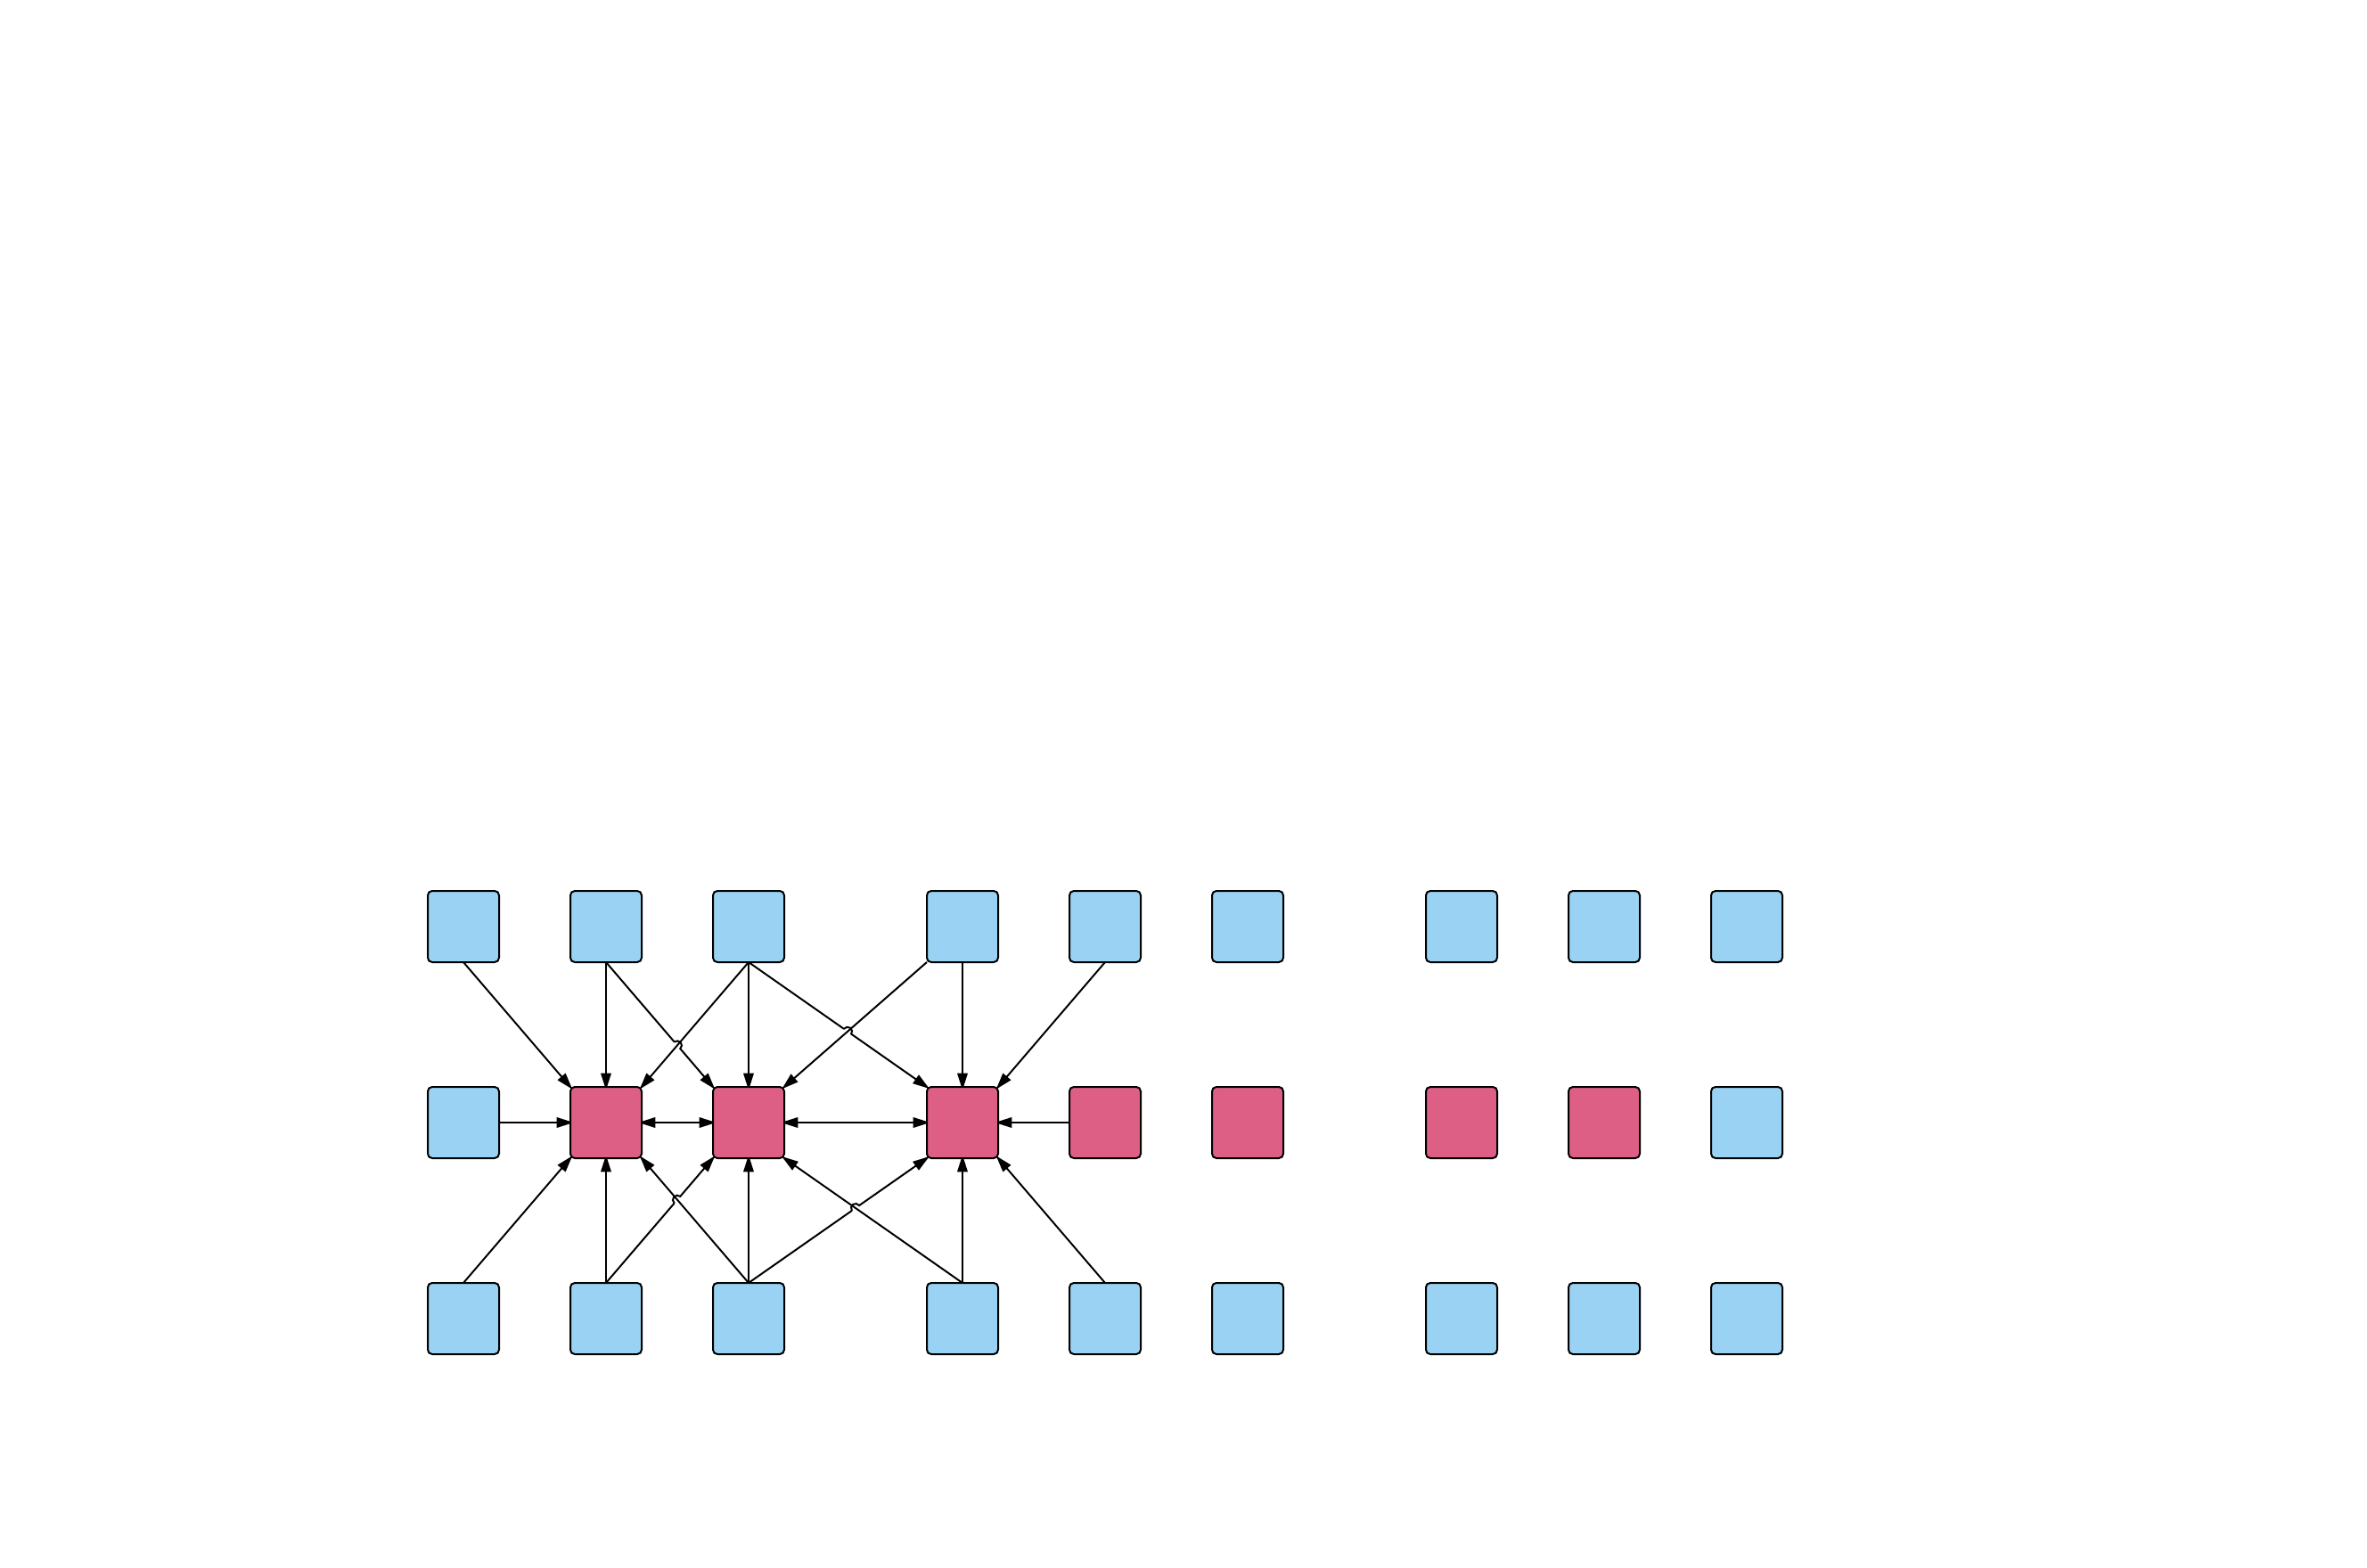
\includegraphics[width=\linewidth]{img/Contexts.png}
    \caption{For each middle pixel, the contexts it applies to neighbouring pixels are denoted by arrows}
    \label{fig:Contexts}
\end{figure}

\begin{figure}[h!]
    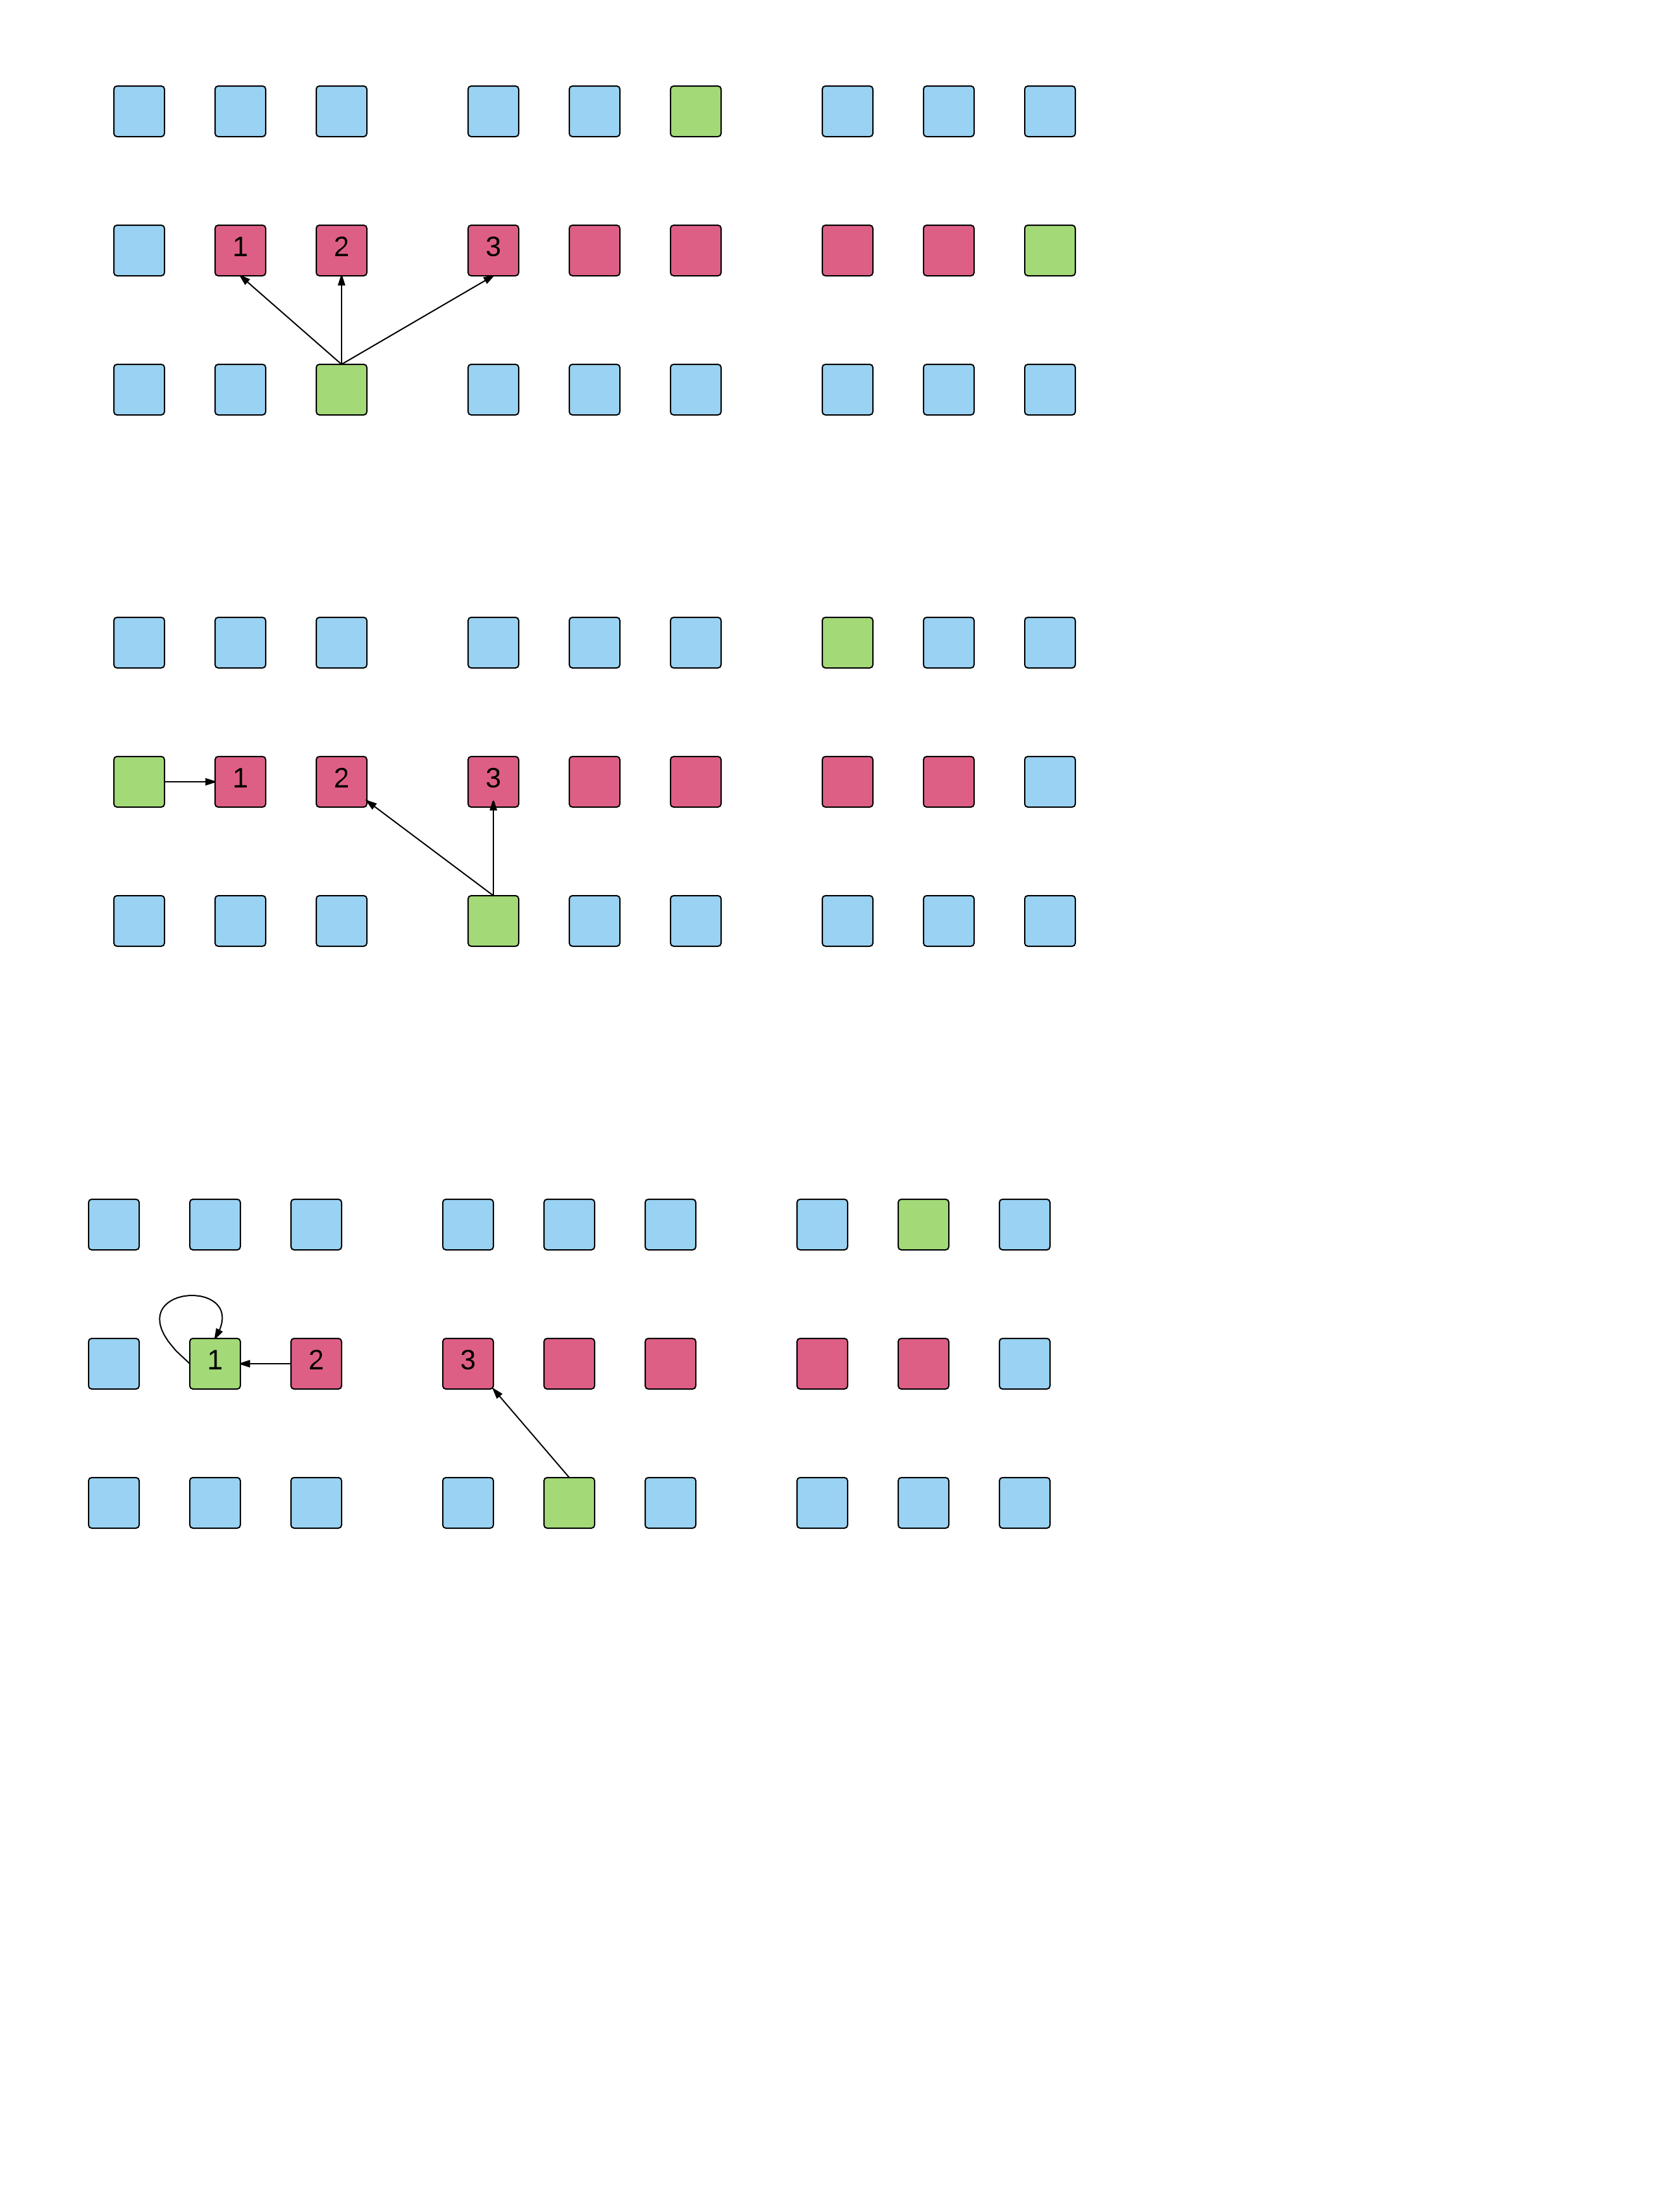
\includegraphics[width=\linewidth]{img/Contexts2.png}
    \caption{For a specific read, marked as green, the contexts it is read in are marked with arrows}
    \label{fig:Contexts}
\end{figure}
\section{Data out}

aaa

We used HDMI!

